\documentclass{report}
\usepackage{Custom_Latex/Summary_Notes/notes}
\usepackage{cancel}
\renewcommand\tabularxcolumn[1]{m{#1}}% for vertical centering text in X column
\usepackage{blkarray}

\begin{document}
\title{R\&A - CW 1}
\author{Maksymilian Mozolewski}
\maketitle
\pagebreak

\section*{3.4}
I am assuming the starting node is A and the goal node is L, and that we are not finding a path, but simply finding node L in BFS/DFS order on the given graph. I am also assuming that by the lexicographic order, you mean that the following is our adjacency matrix:
\begin{center}
    \[
    \begin{blockarray}{ccccccccccc}
    & A & B & C & D & E & F & G & H & I & L \\
    \begin{block}{c(cccccccccc)}
     A & 0 & 1 & 0 & 0 & 3 & 3 & 0 & 0 & 0 & 0\\
     B & 0 & 0 & 1 & 0 & 0 & 0 & 0 & 0 & 0 & 0\\
     C & 0 & 0 & 0 & 1 & 0 & 0 & 0 & 0 & 0 & 0\\
     D & 0 & 1 & 0 & 0 & 0 & 0 & 0 & 0 & 0 & 0\\      
     E & 1 & 0 & 0 & 0 & 0 & 2 & 4 & 0 & 0 & 0\\      
     F & 0 & 0 & 0 & 0 & 0 & 0 & 0 & 1 & 0 & 0\\      
     G & 0 & 0 & 0 & 0 & 0 & 3 & 0 & 0 & 1 & 3\\      
     H & 0 & 0 & 0 & 0 & 0 & 0 & 2 & 0 & 2 & 0\\      
     I & 0 & 0 & 0 & 0 & 0 & 0 & 0 & 0 & 0 & 0\\      
     L & 0 & 0 & 0 & 0 & 2 & 0 & 0 & 0 & 1 & 0\\
    \end{block}
    \end{blockarray}
     \]
\end{center}
And so the successors to each node are returned respecting the order above, and so nodes which appear earlier in the list of successors, are inserted into the appropriate data structure first. I will also be using the iterative implementations to showcase how similar the 2 algorithms are
\subsection*{1.a) - BFS}
I will perform BFS with an iterative approach, by keeping track of a queue of nodes (FIFO, elements dequeued from the left), Any already explored nodes will be ignored at the point when they are generated (I will show them as crossed out nodes in the queue):
\begin{center}
    \begin{tabular}{| c | c | l | c | c |}
    \hline
    iteration & expanded node & queue of generated nodes & explored nodes & goal state generated ?\\ \hline
    0 & - &  \gets A \gets & - & No \\ \hline
    1 & \bd{A} & \gets \bd{B,E,F} \gets & \bd{A} & No \\ \hline
    2 & \bd{B} & \gets E,F,\bd{C} \gets & A,\bd{B} & No \\ \hline
    3 & \bd{E} & \gets F,C,\xcancel{\bd{A}} ,\bd{G} \gets& A,B,\bd{E} & No\\ \hline
    4 & \bd{F} & \gets C,G,\bd{H}  \gets& A,B,E,\bd{F} & No \\ \hline
    5 & \bd{C} & \gets G,H,\bd{D}\gets & A,B,E,F,\bd{C}  & No \\ \hline
    6 & \bd{G} & \gets H,D,\bd{\xcancel{F},{\color{red}L}} \gets& A,B,E,F,C,\bd{G} & \bd{Yes!} \\ \hline
    \end{tabular}
\end{center}

\\

\subsection*{1.b) - DFS }
Similarly like with DFS, I will apply an iterative approach, this time with a stack (a LIFO queue). My earlier assumption here creates interesting behaviour , since the first node inserted will be last to be parsed, the exploring order is effectively reversed to that of BFS in this implementation, therefore to expand the nodes in the same way the recursive algorithm would, I will "reverse" the stack :
\begin{center}
    \begin{tabular}{| c | c | l | c | c |}
    \hline
    iteration & expanded node & stack of generated nodes & explored nodes & goal state expanded ?\\ \hline
    0 & - & \rightarrow A & - & No \\ \hline
    1 & \bd{A} & \rightarrow \bd{B,E,F} & \bd{A} & No\\ \hline
    2 & \bd{B} & \rightarrow \bd{C},E,F & \bd{B},A & No\\ \hline
    3 & \bd{C} & \rightarrow \bd{D},E,F & \bd{C},B,A & No\\ \hline
    4 & \bd{D} & \rightarrow \bd{\xcancel{B}},E,F & - & No\\ \hline
    5 & \bd{E} & \rightarrow \bd{\xcancel{A},\xcancel{F},G},F& \bd{E}& No\\ \hline
    6 & \bd{G} & \rightarrow \bd{\xcancel{F},I,{\color{red}L}},F & \bd{G},E& No\\ \hline
    7 & \bd{I} & \rightarrow {\color{red}L},F & - & No\\ \hline
    8 & \bd{\color{red}L} & \rightarrow F & - & \bd{Yes!} \\ \hline


    \end{tabular}
\end{center}

\subsection*{1.c) - Graph for BFS}
\begin{center}
    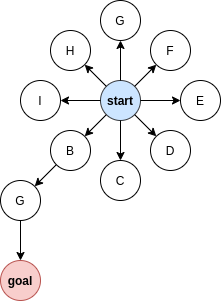
\includegraphics{Custom_Latex/Years/Year2/Semester2/R&A/CW1/Inf2D-Ass1-20/images/BFS.png}
\end{center}
This graph forces the BFS algorithm to look through all of the children around the start node before exploring G, while a DFS algorithm is made to go through only 2 nodes before reaching the goal (assuming recursive implementation, i.e. expanding B first). The graph could also have an infinite number of children from the start, rendering BFS useless.

\subsection*{1.d) - Graph for DFS}
\begin{center}
    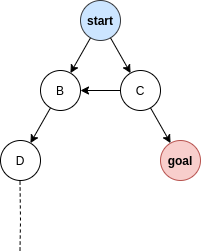
\includegraphics{Custom_Latex/Years/Year2/Semester2/R&A/CW1/Inf2D-Ass1-20/images/DFS.png}
\end{center}
Where the dotted line represents an infinite number of nodes. A BFS solution is not bothered by the inifnite search space, since the solution is present just at depth 2 (would be found after exploring C, 2 nodes). A DFS algorithm however, would be stuck in the depths of the infinite branch and never find the solution (the branch doesn't have to be infinite, just having to reach D first would mean DFS would expand 3 nodes before reaching hte goal state, and underperform.
(assuming the expansion of B first)

\subsection*{1.e)}
DFS and BFS have one main difference, the order in which they expand their frontier. When it comes to implementation, the non-recursive versions of these algorithms differ only in 2 things: 
\begin{itemize}
    \item DFS uses a stack, BFS uses a queue for the frontier, FIFO vs LIFO
    \item BFS checks if a node is a goal node, when it's \emph{generated}, DFS does it when its \emph{expanded}
\end{itemize}
BFS is complete and optimal, while DFS is only complete in finite spaces (and in the graph search version).
Even though BFS is better in that regard, performance wise it requires massive amounts of space compared to DFS ($O(b^{d})$ vs $O(bd)$) and is usually not very practical. The 2 algorithms will fare very differently depending on the types of graphs, and DFS' best case is BFS' worst case and vice versa\par
\subsection*{2.a)}
The optimal depth of that graph is 3, since we can reach the solution node in 3 steps but no less
\subsection*{2.b)}
IDS is DFS but sequentially applied with an increasing depth limit, they both have the same runtime, and space complexity (thanks to the fact that graphs are bottom-heavy). IDS is prefferable whenever the search space is very large, and we don't know anything about the depth at which a solution can be found. Otherwise DFS works better than IDS, due to IDS' overhead incurred when it searches over the same paths multiple times
\section*{4.3}
\subsection*{1.a)}
Every valid heuristic needs to be:
\begin{itemize}
    \item Admissible - meaning that it never overestimates the actual distance/cost to reach the goal node. In the case of straight line distance, it is easy to see, that a straight line is the natural shortest path between any two points, so it cannot overestimate the distance between the goal and the node.
    \item Consistent (required only for graph search) - for every node $n$ and its successor $n^{'}$, if we imagine the segment $n$ to $n^{'}$ as one arm of a triangle, $n^{'}$ to the goal node as another, and $n$ to goal node as the base (see Figure 1), then the triangle must satisfy the triangle inequality: $h(n) \leq c(n,n^{'}) + h(n^{'})$. Now since we know that the lengths of segments $h(n)$ and $h(n')$ are lower bounds on the actual distances they represent, then $h(n)$ cannot possibly be bigger than the other sides of the triangle combined, i.e. there is no path from n through n' to g, shorter than n to g, since that would contradict the fact that $h(n)$ is a lower bound on the distance between those 2 nodes \\
    \begin{figure}[h]
        \centering
        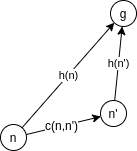
\includegraphics[scale=0.5]{Custom_Latex/Years/Year2/Semester2/R&A/CW1/Inf2D-Ass1-20/images/consistent.png}
        \caption{Triangle inequality}
        \label{fig:my_label}
    \end{figure}
     
\end{itemize}
\subsection*{1.b)}
\begin{tabularx}{\linewidth}{|c | X|}
    \hline
    Heuristics & Problems \\ \hline
    great-circle distance & Shortest railroad between A and B\\ \hline
    total weight of MST$^{1}$ on subgraph of unvisited nodes and current node & travelling salesman problem (least cost hamilton circuit) \\ \hline
    minimum Total hexagonal Manhattan distance of all pawns to closest exits& A game of chineese checkers (10 pawns travelling to opposite side of star-shaped hexagonal board)\\ \hline
\end{tabularx}
\\\\
1 - the minimum spanning tree
\subsection*{2.a)}
The two algorithms are very similar, they both use an evaluation function and choose the order in which they expand nodes in the frontier by selecting the node with smallest evaluation function result when applied to it. The difference is in the choice of evaluation function $f(n)$.
\begin{itemize}
    \item A* uses: $f(n) = h(n) + g(n)$ where $g(n)$ is the total path cost of the node, and $h(n)$ is the heuristic value of the node
    \item Best-first search uses: $f(n) = h(n)$ i.e. it only considers the distance from the goal of each node 
\end{itemize}
This difference causes best-first search to sometimes never find a solution, or find a solution which is not optimal, where as A* always finds the optimal solution. 
\subsection*{2.b)}
I would only need to change the definition of my 'evaluationFunction', and remove the last bit of it i.e "cost graph branch" which would turn my search into a best first search, since that is the only difference between the two
\section*{5.4}
\subsection*{1.}
Done! I will be making some assumptions though!
\subsection*{2.}
The game can be looked at under many angles, but for the purpose of quantifying it, I will assume that we can 'inspect' the game from both sides at the same time, Imagine 2 panels showing both sides of the board. I will assume that only the orientations in which the board is completely vertical count as valid, and each turn must end in the board in a valid orientation. I will also assume that the board is turned 'slowly' as in when the game is turned to the side, and one of its tracks is turned from vertical to horizontal, the discs get 'stay' in place relatively to the top/bottom of the board. When turning from horizontal to vertical, they slide as one would expect.\\\\
Under those conditions, it all boils down to what the player wants to do with the 2 tracks in each of his rotations. For example he could choose to 'tilt' the board and only flip the discs in either of the tracks, he could flip them in both, or not at all. Then he has 16 places to insert the disc, and then another round of rotations. So:\\\\
ways to rotate the discs = ways to flip no tracks + ways to flip one track + ways to flip two tracks
which is:
\begin{equation*}
    = 1 + (2 \cdot 1) + 1 = 4
\end{equation*}
then with 2 rotations and 1 choice for disc the player has $4 \cdot 16 \cdot 4 = \bd{256}$ \bd{different actions} (Go has a branching factor of 250!)
\subsection*{3.}
In considering the feasibility of the alpha beta pruning algorithm, we need to look at the branching factor: b, and the average number of ply's in a single game: d.
we already have the branching factor (assuming no simplifications can be made to the way moves are made). The longest game we can have is at 32 ply, or 16 turns, and the shortest, 7 ply or 3 and a half turns, calculating the average number of moves would be very difficult, so let's just assume it's somewhere in the middle, and let $d = 16$ ply. Assuming optimal move ordering this would lead to $\sqrt{256}^{16} = 1.8446744e+19$ nodes searched. Even if we can look through each node in a single cycle of a single-core 3GHz cpu, this would take us: $3.3333333e-10 \cdot 1.8446744e+19 = 194.85 $ years! And the optimal move ordering would also be very difficult to find, since it's hard to conjure up a general "good moves" list for this game, since they all are very dependent on the situation. With all that in mind, I don't think this approach would be practical (assuming no major improvements/changes to the classic algorithm, apart from move ordering).

\end{document}